% =============================================================================
% thesis.tex
% 修士論文
% スポットインスタンス上の短時間ワークロードにおける
% 実行時刻と分割粒度を考慮した中断対策
%
% 構成:
%   第1章 序論
%   第2章 関連研究
%   第3章 期限条件付き完了可能性          <- main.tex (既発表) を基盤
%   第4章 実測評価                        <- main.tex (既発表)
%   第5章 分割粒度を考慮した実行モデル     <- 新規
%   第6章 実験計画                        <- 新規
%   第7章 結論
%
% コンパイル: lualatex thesis.tex (2回)
% =============================================================================
\documentclass[11pt,a4paper]{ltjsreport}

\usepackage{luatexja}
\usepackage{amsmath,amssymb}
\usepackage{graphicx}
\usepackage{booktabs}
\usepackage{tabularx}
\usepackage{array}
\usepackage{geometry}
\usepackage{caption}
\usepackage{url}
\usepackage[hidelinks]{hyperref}

\geometry{top=30mm,bottom=30mm,left=28mm,right=28mm}
\captionsetup[figure]{labelsep=quad,font=small}
\captionsetup[table]{labelsep=quad,font=small}

% ── 本文で繰り返す記号 ───────────────────────────────────────────────────────
\newcommand{\Fcomp}{F_{\mathrm{comp}}}
\newcommand{\Rlaunch}{R_{\mathrm{launch}}}
\newcommand{\Rint}{R_{\mathrm{int}}}
\newcommand{\Nreq}{N_{\mathrm{req}}}
\newcommand{\Nsucc}{N_{\mathrm{succ}}}
\newcommand{\Nint}{N_{\mathrm{int}}}
\newcommand{\Pspot}{P_{\mathrm{spot}}}
\newcommand{\E}{\mathbb{E}}
\newcommand{\Waste}{\mathrm{Waste}}

\title{\vspace{-10mm}
スポットインスタンス上の短時間ワークロードにおける\\
実行時刻と分割粒度を考慮した中断対策}
\author{那須 渚}
\date{2026年度 修士論文\\[2mm] 同志社大学大学院 理工学研究科}

\begin{document}
\maketitle

% =============================================================================
\chapter*{概要}
\addcontentsline{toc}{chapter}{概要}

スポットインスタンスはクラウド利用コストを大幅に削減できる一方，
提供側の都合により中断される可能性がある．
CI/CD のビルドやテストのような短時間ワークロードでは，
中断が発生するとジョブ全体の再実行が必要となり，
実行時間と利用コストの双方が増加する．

本論文では，短時間ワークロードにおけるスポットインスタンスの信頼性を，
起動可能性ではなく\textbf{期限条件付き完了可能性}
$\Fcomp(d)$ として再定義する．
$\Fcomp(d)$ は，起動に成功したインスタンスが
ワークロード期限 $d$ まで中断されずに利用可能であり続ける割合である．

AWS の 4 リージョン・3 インスタンスタイプを対象として
1 週間（$\Nreq = 2{,}016$）の実測を行い，
$\Fcomp(d)$ がローカル時間帯によって大きく変動することを示した．
計算指向インスタンスでは，Night 期間の $\Fcomp(60) = 0.98$ に対し
Morning 期間では $0.69$ まで低下した．
この結果は，\textbf{実行時刻}が運用上意味のあるスケジューリング要因であることを示す．

しかし時間帯の選択は，最大で 24 時間の待機を要するため，
即時性が求められる CI/CD では適用範囲が限られる．
そこで本論文ではさらに，取得済みデータの再分析を通じて
\textbf{分割粒度}という第二の運用変数を導入する．

再分析の結果，中断ハザード率は経過時間によらずほぼ一定
（0.054--0.130 \%/分）であり，中断が近似的にメモリレスな事象として
振る舞うことが示された．
この性質のもとでは，ジョブを $k$ 分割することで
被中断確率と中断時損失量が同時に低下する．
一方で分割には起動およびチェックポイントのコストが伴うため，
総無駄時間は分割数に対して U 字型となり，
\textbf{最適分割数 $k^{*}$ が存在する}．

さらに感度分析により，$k^{*}$ がチェックポイントコスト $c$ に
極めて敏感であることを明らかにした．
$c = 0$ では $k^{*} = 6$ であるが，$c = 5$ 秒で $k^{*} = 2$ に低下し，
$c \geq 60$ 秒では分割そのものが無効となる．
$c$ は未実測の量であり，提案手法が成立するか否かは $c$ の値に依存する．

以上を踏まえ，本論文では $c$ の実測を最優先とする実験計画を提示する．

% =============================================================================
\tableofcontents
\listoffigures
\listoftables

% =============================================================================
\chapter{序論}

\section{研究背景}

近年，クラウドコンピューティングは企業，研究機関，個人開発者によって
広く利用されている．
クラウド利用の規模が拡大し，高性能な計算資源への需要が増加するにつれて，
その利用コストは多くの利用者にとって重要な課題となっている．

コストを削減する手法の一つに，スポットインスタンスの利用がある．
スポットインスタンスは，クラウドプロバイダが余剰計算資源を
オンデマンドインスタンスより低価格で提供する料金モデルである~\cite{AWSSpot}．
オンデマンドインスタンスと比較して，
数十パーセントから最大約 90\% の割引価格で利用できる~\cite{Lin2022Survey}．
そのため，機械学習やバッチ処理のような大規模計算ワークロードだけでなく，
CI/CD における自動ビルドやテストのように
一時的に計算資源を必要とするワークロードにも利用されている~\cite{Ramesh2025}．

しかしスポットインスタンスは余剰容量に基づいて提供されるため，
クラウド需要が増加した場合や利用可能容量が減少した場合に中断されうる．
この中断を interruption event と呼ぶ．
ワークロードの実行中に interruption event が発生すると，
実行中の処理が完了前に停止する．
特にバッチ処理，機械学習，CI/CD のビルドやテストが中断された場合，
ワークロード全体の再実行が必要となり，
実行時間と利用コストの双方が増加する．

\section{問題意識}

既存のアプローチとしては，価格変動を考慮した入札戦略や，
Spot Placement Score（SPS）のようなプロバイダ固有の
可用性指標に基づく選択が挙げられる~\cite{Garg2025,Katayama2022}．
SPS は，スポットリクエストが成立する可能性を推定する上で有用である．

しかし，CI/CD パイプラインやバッチ処理ジョブのような
短時間ワークロードの利用者にとって，より実用的な問いは
\textbf{スポットインスタンスを起動できるかどうか}だけではなく，
\textbf{ワークロードが完了するまで利用し続けられるかどうか}である．

起動に成功したとしても，ワークロード完了前に中断されれば，
短時間ワークロードは失敗する．
すなわち\textbf{起動時点の可用性}と\textbf{起動後の継続性}は
異なる問題であり，既存指標は前者のみを扱っている．

\section{本研究のアプローチ}

本論文では，スポットインスタンスの信頼性を
\textbf{期限条件付き完了可能性} $\Fcomp(d)$ として再定義し，
これを運用上の意思決定に用いる方法を検討する．

本論文は，二段階の運用変数を扱う．

\paragraph{第一の運用変数：実行時刻．}
多くの CI/CD ジョブやバッチ処理は，比較的柔軟に実行時刻を調整できる．
$\Fcomp(d)$ が時間帯によって異なるならば，
利用者は適切な時間帯を選択することで中断リスクを低減できる．
第 3 章および第 4 章でこれを定式化し，実測により検証する．

\paragraph{第二の運用変数：分割粒度．}
時間帯の選択は最大 24 時間の待機を要するため，
即時性が要求されるワークロードには適用できない．
そこで第 5 章では，ジョブを $k$ 個の断片に分割し，
チェックポイントで接続する手法を導入する．
分割は待機を必要としないため，時刻を選べないジョブにも適用できる．

\section{本論文の貢献}

本論文の貢献は以下の通りである．

\begin{enumerate}
  \item 短時間ワークロードにおけるスポットインスタンスの信頼性を，
        起動可能性やインフラレベルの生存時間ではなく，
        \textbf{期限条件付き完了可能性} $\Fcomp(d)$ として再定義した
        （第 3 章）．
  \item 起動成功と起動後の中断挙動を分離して記録する
        AWS ベースの測定フレームワークを実装し，
        4 リージョン・3 インスタンスタイプ・1 週間の実測を行った
        （第 3 章・第 4 章）．
  \item $\Fcomp(d)$ がローカル時間帯によって大きく変動することを示し，
        実行時刻が運用上のスケジューリング要因となることを明らかにした
        （第 4 章）．
  \item 取得データの再分析により，中断ハザード率が経過時間によらず
        ほぼ一定であること（近似的メモリレス性）を示した（第 5 章）．
  \item この性質に基づき，\textbf{分割粒度}を第二の運用変数とする
        コストモデルを提案し，\textbf{最適分割数 $k^{*}$ が存在する}こと，
        および $k^{*}$ が\textbf{チェックポイントコストに極めて敏感}である
        ことを示した（第 5 章）．
  \item 以上を検証するための実験計画を，
        未実測量であるチェックポイントコストの測定を最優先として設計した
        （第 6 章）．
\end{enumerate}

\section{本論文の構成}

第 2 章では関連研究を整理する．
第 3 章では期限条件付き完了可能性を定義し，測定フレームワークを示す．
第 4 章では実測結果を示し，時間帯による変動を明らかにする．
第 5 章では分割粒度を導入したモデルを提案する．
第 6 章では実験計画を述べる．
第 7 章で本論文をまとめる．

% =============================================================================
\chapter{関連研究}

\section{スポットインスタンスの可用性と時間的変動}

スポットインスタンスの可用性および信頼性については，
これまでに複数の研究が行われている．
Lin ら~\cite{Lin2022Survey} は可用性を向上させる手法を調査し，
チェックポイント，マイグレーション，レプリケーション，スケジューリング
といったアプローチを整理している．
これらの研究は，スポットインスタンスを実用的に利用するうえで
中断リスクが中心的課題であることを示している．

SPS は AWS が提供するプロバイダ固有の指標であり，
インスタンスタイプ，リージョン，必要容量などの条件下で
スポットリクエストが成立する可能性を推定するために用いられる~\cite{AWSSPS}．
Katayama ら~\cite{Katayama2022} はマイグレーション先の選択に SPS を用い，
起動時点の可用性を向上させられることを示した．

Kim ら~\cite{Kim2024SpotInterruption} は，
SPS が時間帯や曜日に応じて周期的に変動し，
survival time と一定の関係を持つことを示している．
ただし同研究では，時間的変動は主にスポット市場の特性として扱われており，
ワークロードの期限に基づく観点からは分析されていない．

本研究は，時間帯を\textbf{短時間ワークロードの実行タイミングを決定する
運用上の変数}として扱う点で，これらと異なる．

\section{スポットインスタンスのデータセットとワークロード指向の利用}

Lee ら~\cite{Lee2022SpotLake} は，SPS，スポット価格，中断率などを
継続的に収集・保存するアーカイブサービス SpotLake を提案した．
同研究では，GPU インスタンスや大規模インスタンスタイプで
可用性が低くなる傾向があること，
可用性がリージョンによって異なることを報告している．

Garg ら~\cite{Garg2025} は AWS Spot Instances に対する
最適化された入札戦略を検討し，
Ramesh と Lennon~\cite{Ramesh2025} は DevOps クラウドワークフローにおける
リザーブドインスタンスとスポットインスタンスの影響を評価している．
これらはスポットインスタンスが CI/CD や DevOps に関連することを示すが，
時間帯と短時間ジョブの完了可能性の関係は十分に検討されていない．

\section{チェックポイントと分割実行}

中断対策としてのチェックポイントは古くから研究されている~\cite{Lin2022Survey}．
機械学習の分野ではエポック単位でのモデル保存が一般的であり，
CI/CD の分野でもテストのシャード分割やビルドキャッシュといった形で
事実上の分割実行が広く行われている．

ただし既存研究の多くは，チェックポイントを
「中断に備えて取るもの」として定性的に扱っており，
\textbf{どの粒度で分割すべきか}という設計問題として
定量的に扱った例は限られている．
本研究は，分割粒度を最適化対象とし，
その最適値がチェックポイントコストによって決まることを示す点で新しい．

\section{本研究の位置づけ}

既存研究に対する本研究の位置づけを表~\ref{tab:related} に示す．

\begin{table}[htbp]
\centering
\caption{関連研究と本研究の位置づけ}
\label{tab:related}
\small
\begin{tabularx}{\textwidth}{@{}lXX@{}}
\toprule
 & \textbf{着目する側面} & \textbf{運用変数} \\
\midrule
SPS~\cite{AWSSPS}，Katayama ら~\cite{Katayama2022}
  & 起動時点の可用性
  & リージョン，AZ \\
\addlinespace
Kim ら~\cite{Kim2024SpotInterruption}
  & 市場の時間的変動，survival time
  & （分析対象であり運用変数ではない） \\
\addlinespace
Lee ら~\cite{Lee2022SpotLake}
  & インフラレベルの可用性データ
  & リージョン，インスタンスタイプ \\
\addlinespace
\textbf{本研究}
  & \textbf{期限条件付き完了可能性}
  & \textbf{実行時刻，分割粒度} \\
\bottomrule
\end{tabularx}
\end{table}

% =============================================================================
\chapter{期限条件付き完了可能性}
\label{chap:fcomp}

\section{問題の定義}

SPS のような既存指標は，スポットリクエストが成立するかどうかを特徴づける．
しかし，起動に成功したインスタンスが
ワークロード完了まで利用可能であり続けるかどうかは示さない．

CI/CD パイプラインやバッチジョブのような短時間ワークロードにとって，
この二つは異なる関心事である．
起動に成功しても完了前に中断されれば，ジョブ全体の再実行が必要となり，
実行時間とコストの双方が増加する．
したがって利用者には，リクエスト成立可能性ではなく
\textbf{期限指向のスポット信頼性}が必要である．

さらに，多くの短時間ワークロードは実行時刻を柔軟に調整できる．
したがって時間帯は中断リスクを低減するための
実行可能な要因となりうる．
しかし既存指標は，この時間帯の影響を期限指向の形で提示しない．

SPS と $\Fcomp(d)$ は，スポット信頼性の異なる側面を捉える
\textbf{相補的な指標}である．
SPS は起動時点の配置可能性を，
$\Fcomp(d)$ は起動後のワークロード固有期限に対する継続性を扱う．

\section{目的}

本章の目的は，起動に成功したスポットインスタンスが
5，10，30，60 分というワークロード期限まで
中断されずに利用可能であり続ける確率を測定し，
それが時間帯，リージョン，インスタンスタイプによって
どのように異なるかを明らかにすることである．

\section{アプローチ}

本研究では実際のアプリケーションレベルのワークロードは実行しない．
代わりに，指定期限まで中断されずに利用可能であることを
\textbf{ワークロード完了可能性の proxy} として用いる．
すなわち，起動に成功したインスタンスが期限 $d$ より前に
中断されなかった場合，観測条件下において
その実行時間要件を持つ短時間ワークロードは完了可能とみなす．

図~\ref{fig:framework} に提案する測定フレームワークを示す．
本フレームワークでは，スケジューラを用いて
スポットインスタンスの起動リクエストを定期的に送信し，
起動結果，稼働状態，中断状態を収集する．

\begin{figure}[htbp]
\centering
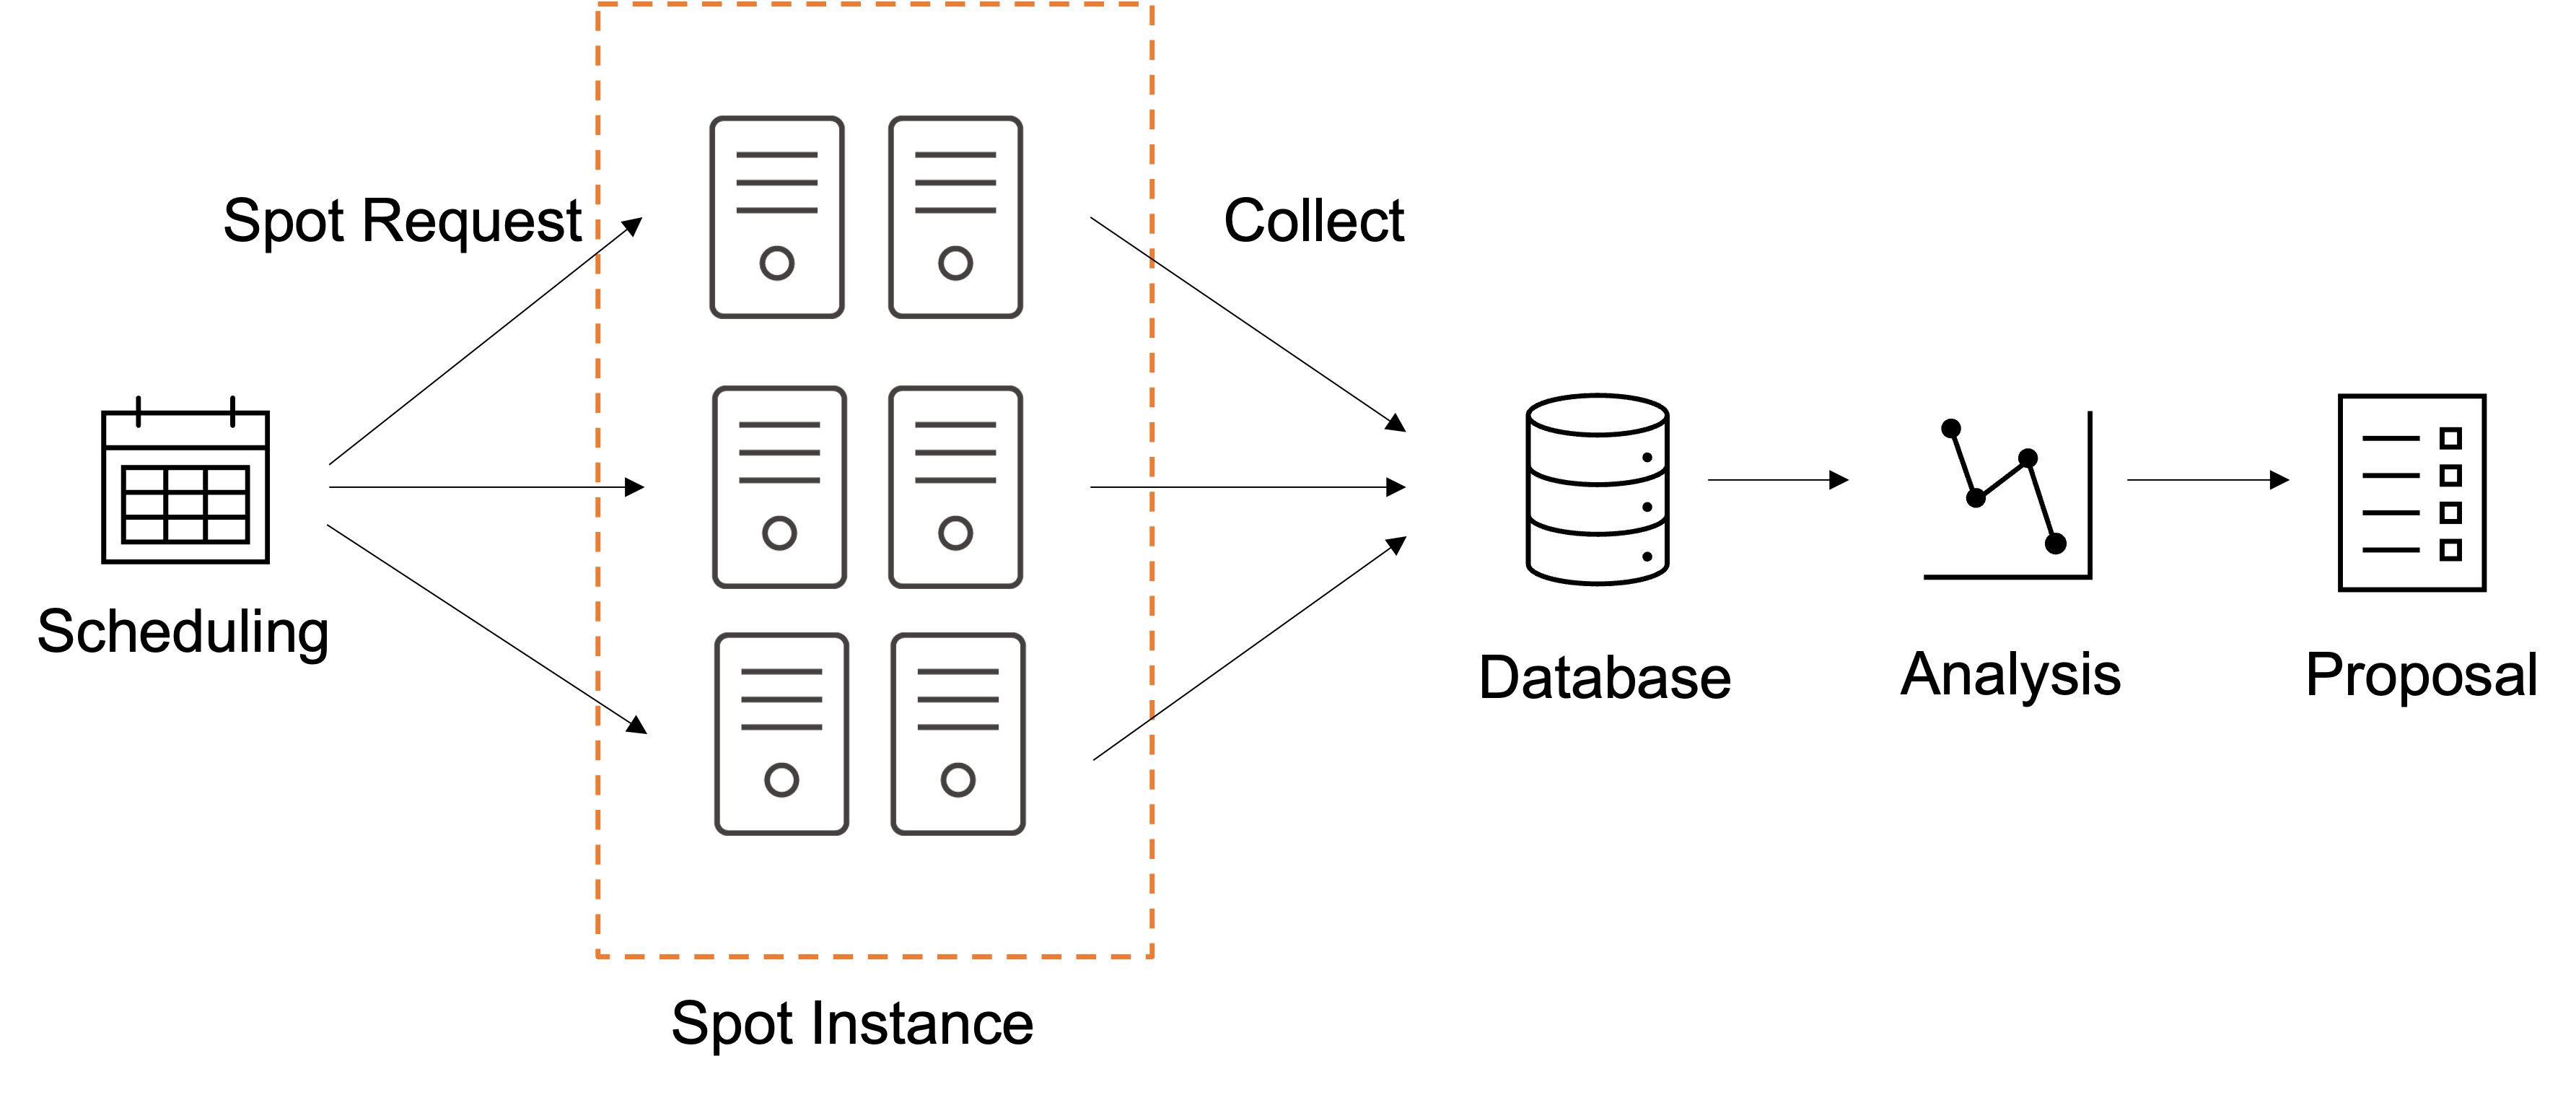
\includegraphics[width=\textwidth]{images/artect.png}
\caption{提案する測定フレームワーク}
\label{fig:framework}
\end{figure}

スケジューラは対象とする各インスタンスタイプに対して
定期的に起動リクエストを送信する．
起動に成功した各インスタンスは 1 時間の固定観測期間にわたって監視される．
この期間中，システムはリクエストが成立したか，
インスタンスがどの程度の時間利用可能であったか，
予定終了時刻より前に interruption event が発生したかを記録する．
観測期間内に中断が発生しなかった場合，
インスタンスはシステムによって終了される．

\section{評価指標の定義}

$\Nreq$ をスポットインスタンスの起動リクエスト数，
$\Nsucc$ を起動に成功したインスタンス数，
$\Nint(d)$ をワークロード期限 $d$ より前に中断された
起動成功インスタンス数とする．

\textbf{起動成功率}を次のように定義する．

\begin{equation}
\Rlaunch = \frac{\Nsucc}{\Nreq}
\label{eq:rlaunch}
\end{equation}

\textbf{期限前中断率}を次のように定義する．

\begin{equation}
\Rint(d) = \frac{\Nint(d)}{\Nsucc}
\label{eq:rint}
\end{equation}

ここで $d$ はワークロード期限である．
本研究では $d = 5, 10, 30, 60$ 分を用いる．
さらに\textbf{期限条件付き完了可能性}を次のように定義する．

\begin{equation}
\boxed{\;\Fcomp(d) = 1 - \Rint(d)\;}
\label{eq:fcomp}
\end{equation}

この指標は，起動に成功したインスタンスのうち
期限 $d$ まで利用可能な状態を維持した割合を表す．
ただしこれは実際のアプリケーションレベルの成功率ではなく，
\textbf{インスタンスの生存に基づく proxy} として解釈すべきである．

式~\eqref{eq:rlaunch} と式~\eqref{eq:rint} を分離して定義することにより，
起動時点の容量不足に起因する失敗と，
起動後に発生する中断とを区別して分析できる．

% =============================================================================
\chapter{実測評価}
\label{chap:eval}

\section{実験方法}

提案フレームワークを AWS 上に実装した．
スケジューラ駆動の Lambda 関数が定期的にスポットインスタンスを起動し，
起動結果，稼働状態，中断イベントをデータベースに記録する．

\paragraph{インスタンスタイプ．}
異なるリソース特性を持つインスタンスタイプ間で中断傾向を比較するため，
3 種類を代表例として選定した~\cite{Pham2018,AWSInstanceTypes}．
仕様を表~\ref{tab:specs} に示す．

\begin{table}[htbp]
\centering
\caption{評価対象インスタンスタイプの仕様。観測スポット価格は観測期間中
（2026年5月19日--25日）に 4 リージョンで記録された平均時間単価（USD/h）である。}
\label{tab:specs}
\small
\begin{tabularx}{\textwidth}{@{}l>{\raggedright\arraybackslash}X>{\raggedright\arraybackslash}X>{\raggedright\arraybackslash}X@{}}
\toprule
 & \textbf{c6a.large} & \textbf{g4dn.xlarge} & \textbf{t3.micro} \\
\midrule
分類 & 計算最適化 & GPU 搭載 & バースト可能汎用 \\
プロセッサ & AMD EPYC (3rd gen) & Intel Xeon (Cascade Lake) & Intel Xeon (burstable) \\
vCPU & 2 & 4 & 2 (burstable) \\
メモリ & 4 GiB & 16 GiB & 1 GiB \\
GPU & --- & 1$\times$ NVIDIA T4 (16 GiB) & --- \\
ローカルストレージ & EBS のみ & 125 GB NVMe SSD & EBS のみ \\
観測スポット価格 & 0.038 & 0.277 & 0.005 \\
\bottomrule
\end{tabularx}
\end{table}

\paragraph{リージョンと時間帯．}
対象リージョンは N.~Virginia (us-east-1)，Tokyo (ap-northeast-1)，
Ireland (eu-west-1)，Singapore (ap-southeast-1) の 4 つである．
各リージョンにおいて，各インスタンスタイプにつき 1 時間に 1 台を起動する．

時間帯の傾向を分析する際，タイムスタンプは
各リージョンのローカル時刻に正規化する．
これにより，各リージョンのローカルな需要サイクルに対して
中断傾向を比較できる．
ローカル 1 日を 6 時間ずつの 4 区間に分割する．

\begin{table}[htbp]
\centering
\caption{ローカル時間帯の区分}
\label{tab:periods}
\small
\begin{tabular}{@{}ll@{}}
\toprule
区分 & ローカル時刻 \\
\midrule
Night     & 00:00--05:59 \\
Morning   & 06:00--11:59 \\
Afternoon & 12:00--17:59 \\
Evening   & 18:00--23:59 \\
\bottomrule
\end{tabular}
\end{table}

スポットリクエストでは最大スポット価格を指定していない．
したがって本実験は，AWS のデフォルトのスポット価格設定における
挙動を観測している．

\paragraph{観測期間．}
実験は 2026 年 5 月 19 日から 5 月 25 日まで実施した．

\paragraph{中断の判定．}
スポット中断と通常のシステム終了を区別するため，
測定システムによって終了されることなく
予定された 1 時間の観測終了前に利用不能となったインスタンスを
中断候補として扱う．

\section{全体結果}

観測期間中，4 リージョン・3 インスタンスタイプにわたり
合計 $\Nreq = 2{,}016$ 件の起動リクエストを送信した．
このうち $\Nsucc = 1{,}950$ 件が正常に起動し，
全体の起動成功率は $\Rlaunch = 96.7\%$ であった．
起動に成功したインスタンスのうち 117 件（$6.0\%$）が
1 時間の観測期間終了前に中断された．

図~\ref{fig:heatmap60} に，ローカル時間帯，リージョン，
インスタンスタイプごとに集計した $\Fcomp(60)$ を示す．

\begin{figure}[htbp]
\centering
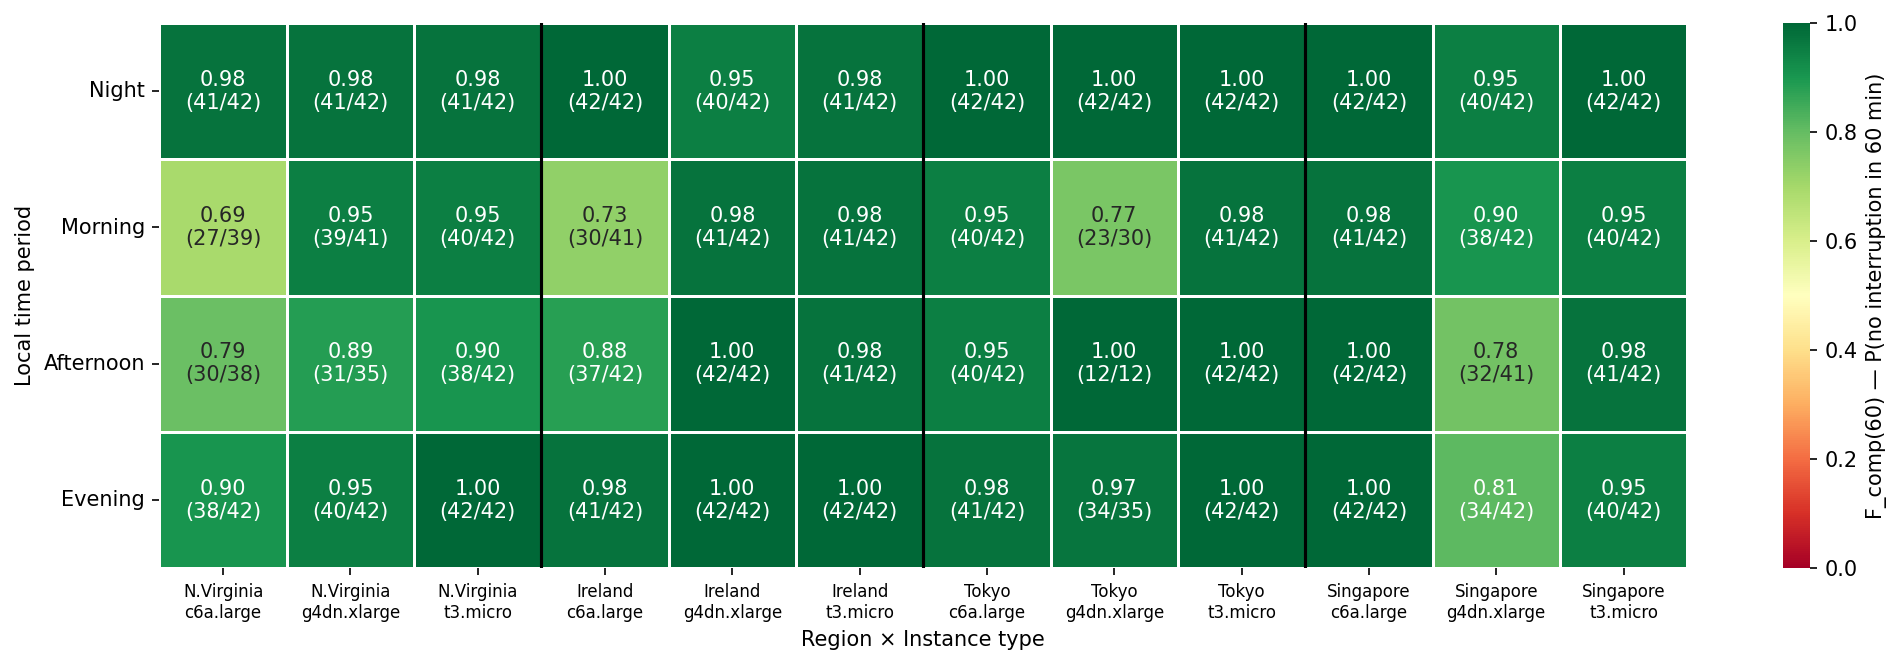
\includegraphics[width=\textwidth]{images/figure1_fcomp60_heatmap.png}
\caption{ローカル時間帯，リージョン，インスタンスタイプ別の
$\Fcomp(60)$。注釈は値とサンプル数（$n_{\mathrm{comp}}/n_{\mathrm{succ}}$）を示す。}
\label{fig:heatmap60}
\end{figure}

t3.micro はすべてのリージョンおよび時間帯において
$\Fcomp(60) \geq 0.95$ を達成しており，
軽量インスタンスは実行タイミングにかかわらず
中断に対して比較的頑健であることを示している．
一方 c6a.large および g4dn.xlarge では時間帯による変動が大きく，
値はおおよそ 0.65 から 1.00 の範囲で変化した．
このことから，計算指向および GPU ベースのインスタンスタイプでは
時間帯が運用上より重要な要因となることが示唆される．

\section{時間帯が完了可能性に与える影響}

図~\ref{fig:multiregion} に，$\Fcomp(60)$ における
時間帯間の変動が最も大きかった 4 つの組み合わせについて，
$d \in \{5, 10, 30, 60\}$ 分に対する $\Fcomp(d)$ を示す．

\begin{figure}[htbp]
\centering
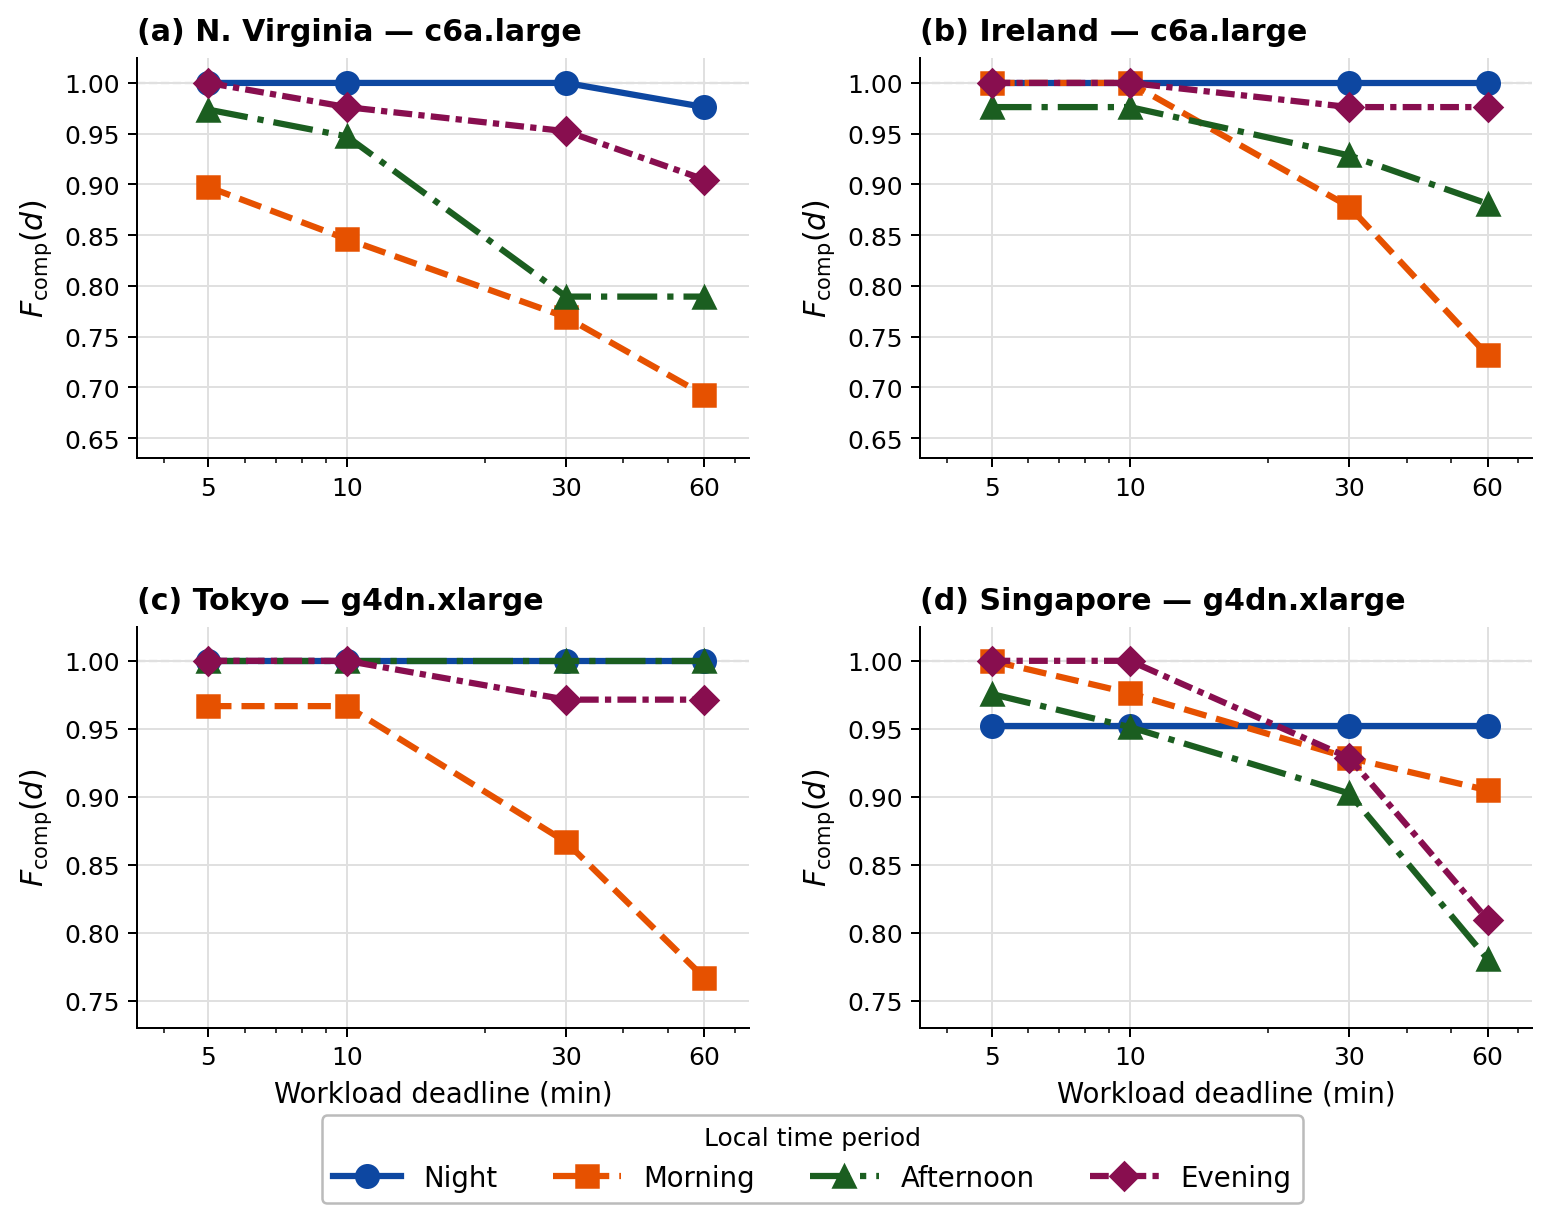
\includegraphics[width=\textwidth]{images/figure2_fcomp_multiregion.png}
\caption{時間帯間の変動が最大であった 4 つのリージョン・インスタンスタイプ
の組み合わせにおける $\Fcomp(d)$。線はローカル時間帯を表し，
横軸は対数スケールである。}
\label{fig:multiregion}
\end{figure}

N.~Virginia の c6a.large では，Night 期間に
$\Fcomp(60) = 0.98$（95\% CI: 0.88--1.00; $n=42$）を達成した一方，
Morning 期間では $\Fcomp(60) = 0.69$（95\% CI: 0.54--0.81; $n=39$）
まで低下し，その差は約 0.29 であった．
二つの信頼区間は重ならず，この差が標本変動に起因する可能性は低い．
最も短い期限である $d = 5$ 分においても，
Morning 期間では既に $\Fcomp(5) = 0.90$（95\% CI: 0.76--0.96）であり，
中断リスクが起動後 5 分以内から蓄積し始めることを示している．

Ireland の c6a.large でも定性的に同様の傾向が見られた．
Night 期間ではすべての期限において
$\Fcomp(60) = 1.00$（95\% CI: 0.92--1.00; $n=42$）を達成した一方，
Morning 期間では $0.73$（95\% CI: 0.58--0.84; $n=41$），
Afternoon 期間では $0.88$（95\% CI: 0.75--0.95; $n=42$）まで低下した．

Tokyo の g4dn.xlarge では Morning 期間に最大の低下が見られ，
$\Fcomp(60) = 0.77$（95\% CI: 0.59--0.88; $n=30$）となった．
Singapore では Afternoon 期間が最低の
$\Fcomp(60) = 0.78$（95\% CI: 0.63--0.88; $n=41$）を示した．

4 つの組み合わせ全体を通じて，Night 期間は一貫して
最も高い，またはそれに近い $\Fcomp(d)$ を示した．
一方で最もリスクの高い時間帯はリージョンによって異なった．

\section{考察}

\subsection{運用上のスケジューリング要因としての時間帯}

結果は，計算指向および GPU ベースのインスタンスタイプにおいて
$\Fcomp(d)$ がローカル時間帯によって大きく変動する一方，
t3.micro ではおおむね安定していることを示す．
最大の差（約 0.29，信頼区間は非重複）は
N.~Virginia の c6a.large における Night と Morning の間で観測された．

観測された傾向は，ローカルなクラウド需要が
日内周期に従うという仮説と整合する．
ローカル夜間には業務利用に起因する計算および GPU 容量への需要が低下し，
スポットインスタンスとして利用可能な余剰容量が増加すると考えられる．
最もリスクの高い時間帯がリージョンによって異なることも
この解釈を支持する．
N.~Virginia と Ireland では Morning が最もリスクが高く，
これは北米および欧州の業務開始時間帯と対応する．
Singapore では Afternoon が最もリスクが高く，
アジア地域の午後の利用ピークと整合する．

\subsection{インスタンスタイプと中断されやすさ}

t3.micro はすべての条件で $\Fcomp(60) \geq 0.95$ を維持し，
c6a.large および g4dn.xlarge と比較して高い安定性を示した．
この違いは，各タイプに対するスポット市場での相対的需要に
起因する可能性がある．
バースト可能な軽量インスタンスは余剰容量をめぐる競合が小さい一方，
計算最適化および GPU 搭載インスタンスは
機械学習やバッチ処理の需要が高く，競合が激しい．
この結果は Lee ら~\cite{Lee2022SpotLake} の知見と整合する．

\subsection{本章の限界}
\label{sec:limit_ch4}

本章の評価にはいくつかの限界がある．

\begin{itemize}
  \item 観測期間は 1 週間に限定されており，
        各時間帯のサンプル数はリージョン・タイプの組み合わせごとに
        約 30--42 である．
        結果は短期的変動を反映している可能性がある．
  \item 中断されない状態を完了可能性の proxy としており，
        実際のアプリケーションレベルのワークロードは実行していない．
        checkpointing，startup overhead，ジョブ間依存といった
        アプリケーション固有の要因は対象外である．
  \item 各組み合わせにつき 1 時間に 1 台のみ起動しているため，
        同時起動の影響やキュー挙動は捉えられていない．
  \item 最大スポット価格を指定していないため，
        デフォルト価格設定下の挙動のみを反映している．
\end{itemize}

\subsection{時間帯選択の適用限界}
\label{sec:timeshift_limit}

本章の結果は，実行時刻が有効な運用変数であることを示した．
しかしこの手法には本質的な制約がある．

Night 期間に実行するためには，到着時刻によっては
最大 24 時間の待機が必要となる．
CI/CD の文脈において，プルリクエストに対するビルドやテストを
夜間まで遅延させることは多くの場合受け入れられない．
すなわち\textbf{時間帯の選択は，実行時刻を柔軟に調整できる
ワークロードにしか適用できない}．

この制約を解消する第二の運用変数を，次章で導入する．

% =============================================================================
\chapter{分割粒度を考慮した実行モデル}
\label{chap:split}

\section{本章のねらい}

第~\ref{chap:eval} 章で示したとおり，実行時刻の選択は有効であるが
待機時間を要するという制約がある（\S\ref{sec:timeshift_limit}）．

本章では，第~\ref{chap:eval} 章で取得したデータを再分析し，
\textbf{分割粒度}という第二の運用変数を導入する．
分割は待機を必要としないため，
実行時刻を選べないワークロードにも適用できる．

ここで重要なのは，第~\ref{chap:fcomp} 章において
$d \in \{5,10,30,60\}$ を\textbf{異なるワークロードの実行時間要件}
として測定した点である．
同じデータを\textbf{同一ジョブを $k$ 分割したときの 1 断片の長さ}
として読み替えることで，新たな解釈が可能となる．
すなわち，追加の測定を行うことなく，
既存データから分割粒度に関する知見を導出できる．

\section{中断の近似的メモリレス性}
\label{sec:memoryless}

分割が有効であるためには，中断の発生様式に関する前提が必要である．
そこで，中断ハザード率が経過時間にどう依存するかを調べた．

経過時間区間ごとに，その区間に入る直前まで生存していた
インスタンス数（リスク集合）で正規化したハザード率を
表~\ref{tab:hazard} および図~\ref{fig:hazard} に示す．

\begin{table}[htbp]
\centering
\caption{経過時間別の中断ハザード率（$\Nsucc = 1{,}950$，中断 117 件）}
\label{tab:hazard}
\small
\begin{tabular}{@{}lrrrr@{}}
\toprule
経過時間 & 中断件数 & リスク集合 & 区間あたり & 単位時間あたり \\
\midrule
0--5 分   & 12 & 1,950 & 0.62\% & 0.123 \%/分 \\
5--10 分  & 11 & 1,938 & 0.57\% & 0.114 \%/分 \\
10--20 分 & 25 & 1,927 & 1.30\% & 0.130 \%/分 \\
20--30 分 & 12 & 1,902 & 0.63\% & 0.063 \%/分 \\
30--40 分 & 14 & 1,890 & 0.74\% & 0.074 \%/分 \\
40--50 分 & 23 & 1,876 & 1.23\% & 0.123 \%/分 \\
50--60 分 & 10 & 1,853 & 0.54\% & 0.054 \%/分 \\
\bottomrule
\end{tabular}
\end{table}

\begin{figure}[htbp]
\centering
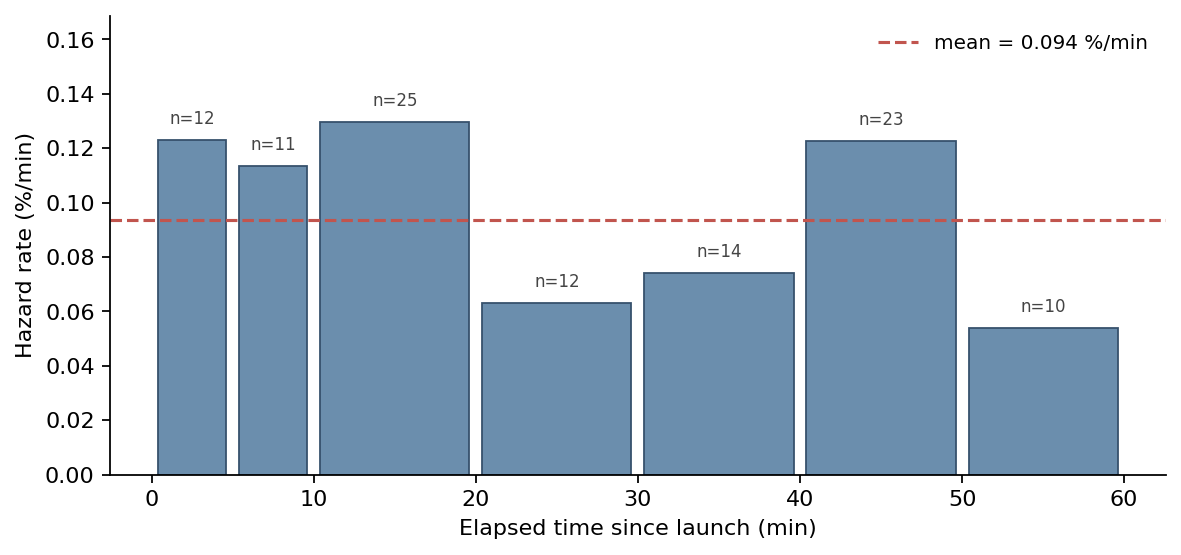
\includegraphics[width=0.85\textwidth]{images/figure3_hazard.png}
\caption{経過時間別の中断ハザード率。単調増加の傾向は見られず，
0.054--0.130 \%/分の範囲で変動する。}
\label{fig:hazard}
\end{figure}

ハザード率は 0.054--0.130 \%/分の範囲で変動するが，
\textbf{経過時間に対する単調増加の傾向は見られない}．
すなわち「長時間稼働したインスタンスほど中断されやすくなる」
という摩耗的な性質は観測されず，
中断は単位時間あたりほぼ一定の確率で発生する
\textbf{近似的にメモリレスな事象}として振る舞う．

\paragraph{この主張の限界．}
中断 117 件という標本数のもとでは，
ハザードの定数性を統計的に強く主張することはできない．
本論文では「単調増加の証拠が得られなかった」という
弱い主張にとどめ，第~\ref{chap:plan} 章の実験で追試する．

\section{分割がもたらす二つの効果}

メモリレス性のもとでは，ジョブを分割することにより
二つの効果が同時に働く．

\paragraph{効果 1：断片あたりの被中断確率の低下．}
稼働時間が短いほど中断に遭遇する機会が減る．
実測された $\Fcomp$ を表~\ref{tab:split_effect} に示す．

\paragraph{効果 2：中断時損失量の低下．}
60 分のジョブが 55 分経過時点で中断されると 55 分が失われるが，
10 分の断片であれば最大 10 分しか失われない
（先行する断片はチェックポイント済みである）．
中断された試行の平均稼働時間
$\bar u(T) = \E[U \mid U < T]$ も，$T$ とともに減少する．

\begin{table}[htbp]
\centering
\caption{断片長 $T$ に対する完了確率と中断時平均損失（全データをプール）}
\label{tab:split_effect}
\small
\begin{tabular}{@{}lrrrr@{}}
\toprule
断片長 $T$ & 60 分 & 30 分 & 10 分 & 5 分 \\
\midrule
$\Fcomp(T)$（点推定）   & 0.945 & 0.969 & 0.988 & 0.994 \\
$\bar u(T)$（中断時損失） & 26.4 分 & 12.7 分 & 4.9 分 & 2.3 分 \\
\bottomrule
\end{tabular}
\end{table}

これら二つが同時に効くため，分割の効果は非線形に大きい．

\section{分割を含むコストモデル}

\subsection{記号と決定変数}

ジョブ $j$ は到着時刻 $t_0$ に到着し，次で特徴づけられる．

\begin{table}[htbp]
\centering
\caption{ジョブの特徴量}
\label{tab:job}
\small
\begin{tabularx}{\textwidth}{@{}llX@{}}
\toprule
記号 & 名称 & 意味 \\
\midrule
$W_j$      & 総計算量 & ジョブ全体の所要時間（分） \\
$D_j$      & 締切     & $t_0 + D_j$ までに完了すべき \\
$k_{\max}$ & 分割上限 & ジョブの性質により定まる分割可能数の上限 \\
\bottomrule
\end{tabularx}
\end{table}

決定変数は\textbf{二つ組} $(t, k)$ である．
$t$ は起動時刻（第~\ref{chap:eval} 章の運用変数），
$k$ は分割数（本章で導入する運用変数）を表す．

分割数 $k$ のとき，1 断片の長さは $T = W_j / k$ となる．

\subsection{総無駄時間}

断片の完了確率を $p(T, \pi)$，中断時の平均損失を $\bar u(T, \pi)$ とする．
ここで $\pi = \pi(t)$ は時刻 $t$ におけるローカル時間帯である
（表~\ref{tab:periods}）．

成功するまで繰り返すときの期待試行回数は $1/p$ であるから，
1 断片あたりのやり直し損失は $(1/p - 1)\,\bar u$ となる．
断片は $k$ 個あり，各断片について起動オーバーヘッド $s$ と
チェックポイントコスト $c$ を要する．
したがって総無駄時間は次式で与えられる．

\begin{equation}
\boxed{\;
\Waste(t,k)
=
\underbrace{k \left( \frac{1}{p(T,\pi(t))} - 1 \right) \bar u(T,\pi(t))}_{\text{やり直し}}
\;+\;
\underbrace{k\,(s + c)}_{\text{起動＋チェックポイント}}
\;}
\label{eq:waste}
\end{equation}

ここで

\begin{itemize}
  \item $s$：インスタンス起動オーバーヘッド。
        第~\ref{chap:eval} 章のデータより\textbf{実測 4.52 秒}
        （中央値 4 秒，95 パーセンタイル 6 秒）。
  \item $c$：チェックポイントの保存および復元コスト。
        \textbf{本論文では未実測であり，第~\ref{chap:plan} 章の測定対象とする}。
\end{itemize}

第 1 項は $k$ の増加とともに減少し，第 2 項は $k$ に比例して増加する．
したがって $\Waste$ は $k$ に対して U 字型となる．

\subsection{最適化問題}

以上より，提案手法は次の制約付き最適化問題として記述される．

\begin{equation}
\begin{aligned}
\min_{t,\,k}\quad
  & \Waste(t,k) && \text{（総無駄時間）} \\[3pt]
\text{s.t.}\quad
  & t \in [\,t_0,\; t_0 + D_j - W_j\,] && \text{（締切）} \\[2pt]
  & k \in \{1, 2, \ldots, k_{\max}\}   && \text{（分割可能性）} \\[2pt]
  & p(W_j/k,\, \pi(t)) \geq p_{\min}   && \text{（信頼性下限）}
\end{aligned}
\label{eq:opt}
\end{equation}

探索空間は $24 \times k_{\max}$ 程度であり，全列挙により厳密に解ける．

\subsection{第~\ref{chap:fcomp} 章との関係}

$k = 1$ に固定すると，式~\eqref{eq:waste} は

\begin{equation}
\Waste(t,1) = \left( \frac{1}{\Fcomp(W_j)} - 1 \right) \bar u + s + c
\end{equation}

となり，第~\ref{chap:fcomp} 章で定義した $\Fcomp$ に帰着する．
すなわち\textbf{第~\ref{chap:fcomp} 章のモデルは，
本章のモデルにおいて $k=1$ とした特殊ケース}である．

\section{最適分割数の存在}

式~\eqref{eq:waste} を既存データに適用し，
$k$ に対する総無駄時間を算出した．
推定には Wilson 95\% 下側信頼限界を用い，
標本数が少ないことによる楽観的推定を抑制した．

結果を表~\ref{tab:ucurve} に示す（$c = 0$ の場合）．

\begin{table}[htbp]
\centering
\caption{分割数 $k$ に対する総無駄時間（$W_j = 60$ 分，$c = 0$，Wilson LCB）}
\label{tab:ucurve}
\small
\begin{tabular}{@{}rrrrrrr@{}}
\toprule
$k$ & 断片長 & $p_{\mathrm{LCB}}$ & やり直し & 起動 & \textbf{合計} & vs $k{=}1$ \\
\midrule
1  & 60.0 分 & 0.9341 & 1.86 分 & 0.08 分 & \textbf{1.94 分} & --- \\
2  & 30.0 分 & 0.9606 & 1.04 分 & 0.15 分 & \textbf{1.19 分} & $-39\%$ \\
3  & 20.0 分 & 0.9675 & 0.97 分 & 0.23 分 & \textbf{1.19 分} & $-38\%$ \\
4  & 15.0 分 & 0.9728 & 0.91 分 & 0.30 分 & \textbf{1.21 分} & $-38\%$ \\
\textbf{6}  & \textbf{10.0 分} & 0.9824 & 0.53 分 & 0.45 分 & \textbf{0.98 分} & $\mathbf{-50\%}$ \\
10 & 6.0 分  & 0.9880 & 0.34 分 & 0.75 分 & \textbf{1.09 分} & $-44\%$ \\
12 & 5.0 分  & 0.9893 & 0.30 分 & 0.90 分 & \textbf{1.20 分} & $-38\%$ \\
20 & 3.0 分  & 0.9906 & 0.39 分 & 1.51 分 & \textbf{1.90 分} & $-2\%$ \\
60 & 1.0 分  & 0.9980 & 0.00 分 & 4.52 分 & \textbf{4.52 分} & $+133\%$ \\
\bottomrule
\end{tabular}
\end{table}

$k = 6$（10 分ごとの分割）において総無駄時間は最小となり，
$k=1$ と比較して $50\%$ の削減が得られる．
一方 $k = 60$（1 分ごと）では起動コストが支配的となり，
分割しない場合よりも $133\%$ 悪化する．

すなわち\textbf{「細かく切るほど良い」という直観は誤りであり，
最適分割数 $k^{*}$ が存在する}．

\section{チェックポイントコストに対する感度}
\label{sec:sensitivity}

表~\ref{tab:ucurve} は $c = 0$ を仮定した理想値である．
実際にはチェックポイントの保存と復元に時間を要する．
$c$ を変化させたときの $k^{*}$ を表~\ref{tab:sensitivity} および
図~\ref{fig:ucurve} に示す．

\begin{table}[htbp]
\centering
\caption{チェックポイントコスト $c$ に対する最適分割数 $k^{*}$ の感度。
各セルは総無駄時間（分）を表し，太字は各行の最小値を示す。}
\label{tab:sensitivity}
\small
\begin{tabular}{@{}rrrrrrc@{}}
\toprule
$c$ (秒) & $k{=}1$ & $k{=}2$ & $k{=}4$ & $k{=}6$ & $k{=}12$ & $\mathbf{k^{*}}$ \\
\midrule
0   & 1.94 & 1.19 & 1.21 & \textbf{0.98} & 1.20 & \textbf{6} \\
5   & 2.02 & \textbf{1.36} & 1.54 & 1.48 & 2.20 & \textbf{2} \\
10  & 2.11 & \textbf{1.52} & 1.88 & 1.98 & 3.20 & \textbf{2} \\
30  & 2.44 & \textbf{2.19} & 3.21 & 3.98 & 7.20 & \textbf{2} \\
60  & \textbf{2.94} & 3.19 & 5.21 & 6.98 & 13.20 & \textbf{1} \\
120 & \textbf{3.94} & 5.19 & 9.21 & 12.98 & 25.20 & \textbf{1} \\
\bottomrule
\end{tabular}
\end{table}

\begin{figure}[htbp]
\centering
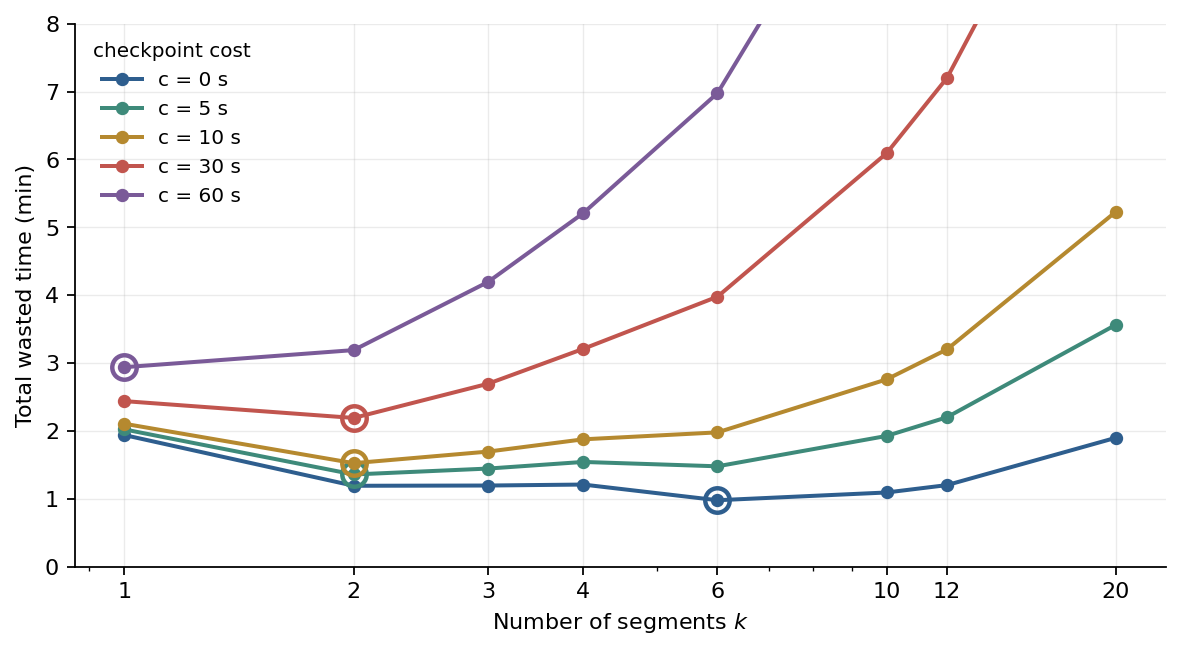
\includegraphics[width=0.9\textwidth]{images/figure4_ucurve.png}
\caption{分割数に対する総無駄時間の U 字カーブ。
各曲線はチェックポイントコスト $c$ の値に対応し，
二重丸は各曲線の最小点 $k^{*}$ を示す。
$c$ の増加とともに $k^{*}$ は左へ移動する。}
\label{fig:ucurve}
\end{figure}

この結果は本研究にとって決定的である．

\begin{itemize}
  \item わずか 5 秒のチェックポイントコストで
        $k^{*}$ は 6 から 2 へ低下する．
  \item $c \geq 60$ 秒では $k^{*} = 1$ となり，
        \textbf{分割そのものが無効}となる．
\end{itemize}

すなわち\textbf{提案手法が成立するか否かは $c$ の値によって決まる}．
$c$ は本論文では未実測であり，
第~\ref{chap:plan} 章の実験における最優先の測定対象となる．

\section{実行時刻との併用}

実行時刻（第~\ref{chap:eval} 章）と分割粒度（本章）は
独立した運用変数である．
両者を組み合わせた場合の総無駄時間を
表~\ref{tab:period_k} および図~\ref{fig:period_k} に示す．

\begin{table}[htbp]
\centering
\caption{ローカル時間帯と分割数の組み合わせによる総無駄時間（分，$c=0$，Wilson LCB）}
\label{tab:period_k}
\small
\begin{tabular}{@{}lrrrr@{}}
\toprule
時間帯 & $k{=}1$ & $k{=}2$ & $k{=}6$ & $k{=}12$ \\
\midrule
Night     & 1.09 & 0.73 & \textbf{0.60} & 1.19 \\
Morning   & \textbf{3.81} & 2.13 & \textit{1.62} & 1.72 \\
Afternoon & 2.58 & 2.18 & 1.69 & 1.53 \\
Evening   & 2.05 & 1.00 & 1.07 & 0.90 \\
\bottomrule
\end{tabular}
\end{table}

\begin{figure}[htbp]
\centering
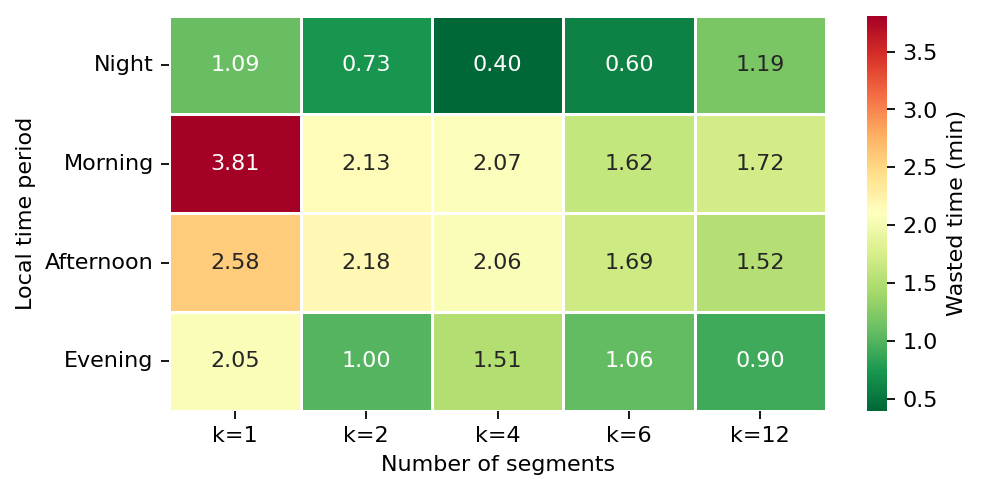
\includegraphics[width=0.75\textwidth]{images/figure5_period_k.png}
\caption{ローカル時間帯と分割数の組み合わせによる総無駄時間。
色が濃いほど無駄時間が大きい。}
\label{fig:period_k}
\end{figure}

表~\ref{tab:period_k} から次の三点が読み取れる．

\begin{enumerate}
  \item 最悪条件（Morning，$k{=}1$）の 3.81 分に対し，
        最良条件（Night，$k{=}6$）は 0.60 分であり，
        $84\%$ の削減となる．
  \item \textbf{実行時刻を選べない場合でも}，Morning において
        $k{=}6$ とすれば 3.81 分から 1.62 分へ $57\%$ 削減される．
        これは時刻選択に匹敵する効果を\textbf{待機時間ゼロ}で得られることを意味する．
  \item 両者は独立に作用するため，併用により最大の効果が得られる．
\end{enumerate}

\section{比較対象とする戦略}

第~\ref{chap:plan} 章の実験では，式~\eqref{eq:opt} の制約を変化させることで
定義される以下の戦略を比較する．

\begin{table}[htbp]
\centering
\caption{比較する戦略}
\label{tab:strategies}
\small
\begin{tabularx}{\textwidth}{@{}llX@{}}
\toprule
戦略 & $(t, k)$ & 位置づけ \\
\midrule
B0: Naive        & $t_0$ 固定，$k{=}1$ & 素朴な実行（ベースライン） \\
B1: 時刻のみ     & $t$ 自由，$k{=}1$   & \textbf{第~\ref{chap:eval} 章の手法} \\
B2: 分割のみ     & $t_0$ 固定，$k$ 自由 & 待機時間ゼロ \\
B3: 併用（提案） & $t$ 自由，$k$ 自由   & 完全版 \\
\bottomrule
\end{tabularx}
\end{table}

B1 と B2 を分離することにより，
実行時刻と分割粒度それぞれの寄与を独立に評価できる．

\section{補足：リージョン選択について}

第~\ref{chap:eval} 章の考察では，実行時刻を調整できない場合の代替として
リージョン選択に言及した．
しかし既存データを用いた検討の結果，
\textbf{コスト最小化を目的とする限りリージョン選択は機能しない}
ことが判明した．

表~\ref{tab:region_price} に示すとおり，
リージョン間の価格差（34--41\%）が
信頼性の差（期待課金時間にして数パーセント）を大きく上回る．
このため常に最安リージョンが選択され，
リージョンを自由に選べる戦略は
リージョンを固定した戦略と同一の結果となった．

\begin{table}[htbp]
\centering
\caption{c6a.large のリージョン別観測スポット価格}
\label{tab:region_price}
\small
\begin{tabular}{@{}lrr@{}}
\toprule
リージョン & 価格 (USD/h) & N.~Virginia 比 \\
\midrule
N.~Virginia & 0.0295 & --- \\
Singapore   & 0.0394 & $+34\%$ \\
Ireland     & 0.0400 & $+36\%$ \\
Tokyo       & 0.0417 & $+41\%$ \\
\bottomrule
\end{tabular}
\end{table}

この否定的結果は，実行時刻と分割粒度という
二つの運用変数に注力する本研究の方針を支持するものである．

% =============================================================================
\chapter{実験計画}
\label{chap:plan}

\section{実験の目的と優先順位}

\S\ref{sec:sensitivity} で示したとおり，
提案手法の成否はチェックポイントコスト $c$ に依存する．
したがって実験の目的を以下の優先順位で設定する．

\begin{table}[htbp]
\centering
\caption{実験の目的と優先順位}
\label{tab:objectives}
\small
\begin{tabularx}{\textwidth}{@{}clX@{}}
\toprule
優先 & 目的 & 理由 \\
\midrule
1 & \textbf{$c$ の実測}
  & $k^{*}$ を決定する最重要パラメータであり未知。
    $c \geq 60$ 秒であれば提案手法の前提が崩れる \\
\addlinespace
2 & U 字カーブの検証
  & 式~\eqref{eq:waste} の妥当性検証 \\
\addlinespace
3 & 中断の独立性の検証
  & 期待試行回数 $1/p$ の前提の検証 \\
\addlinespace
4 & 実行時刻との併用効果
  & 第~\ref{chap:eval} 章との接続 \\
\bottomrule
\end{tabularx}
\end{table}

\section{対象ワークロードの選定}

\subsection{選定基準}

\begin{itemize}
  \item 実行時間が 30 分以上であること
        （短いと $\Fcomp > 0.99$ となり差が検出できない）
  \item チェックポイントが実装可能であること
  \item $c$ が現実的に測定できること
  \item 中断率の高い条件を選択できること
\end{itemize}

\subsection{候補の比較}

$c$ の大きさが対照的な二つのワークロードを選定する．

\begin{table}[htbp]
\centering
\caption{対象ワークロードの候補}
\label{tab:usecases}
\small
\begin{tabularx}{\textwidth}{@{}lXX@{}}
\toprule
 & \textbf{A: 機械学習の学習} & \textbf{B: CI/CD テスト} \\
\midrule
分割の単位   & エポック & テストシャード \\
チェックポイント & モデルの保存・復元 & 結果 JSON の保存 \\
想定 $c$     & \textbf{30--120 秒}（数百 MB） & \textbf{1--5 秒}（数 KB） \\
予測 $k^{*}$ & \textbf{1--2（分割は無効）} & \textbf{2--6（分割が有効）} \\
インスタンス & g4dn.xlarge & c6a.large \\
中断率       & 高い & 低い \\
既発表との接続 & 弱い & \textbf{強い} \\
\bottomrule
\end{tabularx}
\end{table}

$c$ が対照的であるため，両者を実施することで
\textbf{どのようなワークロードであれば分割が有効か}という
一般的な指針が得られる．
これは単一ワークロードによる評価よりも強い主張となる．

一方のみを実施する場合は B（CI/CD テスト）を選択する．
第~\ref{chap:eval} 章との接続が強く，
コストが約 1/10 であり，$c$ が小さく分割が有効となる可能性が高いためである．

\section{実験 1：チェックポイントコストの実測}

\paragraph{目的．}
$c$ を実測し，図~\ref{fig:ucurve} の理論曲線上で
$k^{*}$ を確定する．

\paragraph{方法．}
中断のない環境において分割数 $k$ を変化させ，
純粋なオーバーヘッドのみを測定する．
各断片についてチェックポイントの保存時間，
復元時間，インスタンス起動時間を記録し，
$c = \text{保存} + \text{復元}$ の平均を求める．

\paragraph{規模．}
$k \in \{1,2,4,6,12\}$ をそれぞれ 10 回実施する．
断片数の合計は $(1+2+4+6+12)\times 10 = 250$ 本，
総計算時間は約 50 時間である．
中断の発生を待つ必要がないため \textbf{1--2 日で完了}する．

\paragraph{意義．}
この実験の結果のみで，理論曲線上の $k^{*}$ が確定する．
以降の実験設計はこの結果を踏まえて確定させる．

\section{実験 2：U 字カーブの検証}

\paragraph{目的．}
実測された $c$ のもとで予測される $k^{*}$ が，
実際に総無駄時間を最小化するかを検証する．

\paragraph{方法．}
中断が発生しやすい条件として
N.~Virginia，c6a.large，Morning 期間を選択する
（第~\ref{chap:eval} 章において $\Fcomp(60) = 0.69$ と最低値を記録）．
$k \in \{1,2,4,6,12\}$ を各 24 回／日，14 日間実施する．
中断された場合は当該断片のみを再実行し，
先行する断片はチェックポイントから復元する．

\paragraph{測定項目．}
総課金時間，やり直し回数，完了までの実時間．

\paragraph{規模．}
$5 \times 24 \times 14 = 1{,}680$ 本の実行．

\section{実験 3：中断の独立性の検証}

\paragraph{目的．}
「中断された直後の再試行も同じ確率 $p$ で成功する」
という仮定を検証する．

式~\eqref{eq:waste} における期待試行回数 $1/p$ は，
各試行が独立であることを前提としている．
しかし中断は容量逼迫時に発生すると考えられるため，
直後の再試行はより失敗しやすい可能性がある．
その場合 $p$ は過大評価であり，
分割の効果も割り引いて解釈する必要がある．

\paragraph{方法．}
中断を検知した場合に即座に同一条件で再起動し，
2 回目の成否を記録する．
1 回目の $p$ と 2 回目の $p$ を比較する．

\paragraph{規模．}
中断 50 件の収集を目標とする．
中断率 6\% のもとでは約 830 回の起動を要する．
\textbf{実験 2 と同一の実行に相乗りできる}
（実験 2 で中断された断片の再試行結果を記録すればよい）．

\section{実験 4：実行時刻との併用}

\paragraph{目的．}
第~\ref{chap:eval} 章の手法（実行時刻）と
第~\ref{chap:split} 章の手法（分割粒度）の
寄与を分離して評価する．

\paragraph{方法．}
表~\ref{tab:strategies} の B0--B3 を比較する．
表~\ref{tab:period_k} に基づく予測値は
3.81 / 1.09 / 1.62 / 0.60 分である．

\paragraph{期待される知見．}
B2（分割のみ）が B1（時刻のみ）に匹敵すれば，
\textbf{待機を伴わずに同等の効果が得られる}ことが実証される．

\section{実験規模のまとめ}

\begin{table}[htbp]
\centering
\caption{実験の規模とコスト（c6a.large を想定）}
\label{tab:exp_scale}
\small
\begin{tabularx}{\textwidth}{@{}llrX@{}}
\toprule
実験 & 期間 & コスト & 得られるもの \\
\midrule
1: $c$ の実測   & \textbf{1--2 日} & \$1.5 & \textbf{$k^{*}$ の確定} \\
2: U 字検証     & 2 週間 & \$25 & モデルの妥当性 \\
3: 独立性       & 実験 2 に相乗り & \$0 & 前提の検証 \\
4: 併用         & 2 週間 & \$25 & 第~\ref{chap:eval} 章との接続 \\
\midrule
\textbf{合計}   & \textbf{約 1 か月} & \textbf{約 \$52} & \\
\bottomrule
\end{tabularx}
\end{table}

機械学習ワークロード（実験 1 のみ g4dn.xlarge で追加実施）を
含めても約 \$70 である．

\section{実装方針}

第~\ref{chap:eval} 章で構築した測定フレームワークを流用する．
変更点を表~\ref{tab:impl} に示す．

\begin{table}[htbp]
\centering
\caption{既存実装からの変更点}
\label{tab:impl}
\small
\begin{tabularx}{\textwidth}{@{}lX@{}}
\toprule
既存要素 & 変更内容 \\
\midrule
起動 Lambda & user-data の待機処理を実ワークロードに置換 \\
中断検知ループ & そのまま流用（インスタンスメタデータの監視） \\
記録テーブル & 断片番号，分割数，保存時間，復元時間を追加 \\
スケジューラ & 「断片完了後に次の断片を起動」する連鎖を追加 \\
\bottomrule
\end{tabularx}
\end{table}

チェックポイントの保存先はオブジェクトストレージとし，
各断片は直前の断片が保存した状態を読み込み，
処理後に次の状態を書き出す．

\section{想定される結果}

実験 1 の結果に応じて，導かれる結論は以下のように分岐する．
\textbf{いずれの場合も報告価値のある結果となる}．

\begin{table}[htbp]
\centering
\caption{チェックポイントコストの実測値に応じた結論}
\label{tab:outcomes}
\small
\begin{tabularx}{\textwidth}{@{}llX@{}}
\toprule
$c$ の実測値 & $k^{*}$ & 導かれる結論 \\
\midrule
$c < 5$ 秒 & 4--6
  & 分割は実行時刻の選択を代替できる。最適粒度は約 10 分 \\
\addlinespace
$5 \leq c < 30$ 秒 & 2
  & 分割は有効だが粗く切るべきであり，細分化は逆効果 \\
\addlinespace
$30 \leq c < 60$ 秒 & 2
  & 分割による利得は限定的 \\
\addlinespace
$c \geq 60$ 秒 & 1
  & \textbf{分割は成立しない。実行時刻の選択が唯一の手段であり，
    第~\ref{chap:eval} 章の手法の価値が補強される} \\
\bottomrule
\end{tabularx}
\end{table}

\section{リスクと対策}

\begin{table}[htbp]
\centering
\caption{想定されるリスクと対策}
\label{tab:risks}
\small
\begin{tabularx}{\textwidth}{@{}XXX@{}}
\toprule
リスク & 影響 & 対策 \\
\midrule
$c$ が大きく分割が無効
  & 提案の前提が崩れる
  & 実験 1 を最優先し 1--2 日で判明させる。
    無効でも否定的結果として報告する \\
\addlinespace
中断が十分に集まらない
  & 実験 2 の検出力不足
  & 中断率が最も高い条件に集中させる \\
\addlinespace
ハザード一定が偽
  & メモリレス性の前提が崩れる
  & 実験で追試する。標本数 117 の限界を明記済み
    （\S\ref{sec:memoryless}） \\
\addlinespace
独立性が成立しない
  & $p$ が過大評価となる
  & 実験 3 で検証し，必要なら条件付き確率へ修正する \\
\addlinespace
観測期間と実験期間の市場変化
  & 予測が外れる
  & 実験期間中に $\Fcomp$ を再測定し比較する \\
\bottomrule
\end{tabularx}
\end{table}

% =============================================================================
\chapter{結論}

\section{本論文のまとめ}

本論文では，スポットインスタンス上の短時間ワークロードにおける
中断対策を，二つの運用変数の観点から論じた．

第~\ref{chap:fcomp} 章では，スポットインスタンスの信頼性を
起動可能性ではなく\textbf{期限条件付き完了可能性} $\Fcomp(d)$ として
再定義し，起動成功と起動後の中断挙動を分離して記録する
測定フレームワークを示した．

第~\ref{chap:eval} 章では，AWS の 4 リージョン・3 インスタンスタイプを
対象とした 1 週間の実測（$\Nreq = 2{,}016$）により，
$\Fcomp(d)$ がローカル時間帯によって大きく変動することを示した．
計算指向インスタンスでは Night 期間の $0.98$ に対し
Morning 期間では $0.69$ まで低下し，
\textbf{実行時刻}が運用上意味のある変数であることを明らかにした．
一方で，この手法は最大 24 時間の待機を要するという制約を持つ．

第~\ref{chap:split} 章では，取得済みデータの再分析により
中断ハザード率が経過時間によらずほぼ一定であることを示し，
この近似的メモリレス性に基づいて\textbf{分割粒度}を
第二の運用変数として導入した．
分割数 $k$ を含むコストモデルを定式化し，
総無駄時間が $k$ に対して U 字型となること，
すなわち\textbf{最適分割数 $k^{*}$ が存在する}ことを示した．
さらに感度分析により，$k^{*}$ が
\textbf{チェックポイントコスト $c$ に極めて敏感}であり，
$c \geq 60$ 秒では分割が無効となることを明らかにした．

第~\ref{chap:plan} 章では，$c$ の実測を最優先とする実験計画を示した．

\section{本研究の意義}

本研究の意義は以下の三点である．

\begin{enumerate}
  \item スポットインスタンスの信頼性を，
        プロバイダ固有の不透明な指標ではなく，
        直接観測された起動・中断記録のみから算出される
        \textbf{解釈可能な指標}として定式化した．
  \item 実行時刻という既知の変数に加え，
        \textbf{分割粒度}という新たな運用変数を導入し，
        待機を伴わない中断対策の可能性を示した．
  \item 「細かく分割するほど良い」という直観に反し，
        \textbf{最適分割数が存在し，それがチェックポイントコストに
        支配される}ことを定量的に示した．
\end{enumerate}

\section{今後の課題}

\begin{itemize}
  \item 第~\ref{chap:plan} 章の実験計画の実施，
        とりわけチェックポイントコスト $c$ の実測
  \item 観測期間の延長による，季節変動を含む長期的傾向の把握
  \item 中断のメモリレス性に関する，より大きな標本に基づく検証
  \item SPS など既存のプロバイダ固有指標との定量的比較
  \item 実際の CI/CD ワークロードおよび機械学習ワークロードにおける評価
\end{itemize}

% =============================================================================
\chapter*{謝辞}
\addcontentsline{toc}{chapter}{謝辞}

本研究を進めるにあたり，終始丁寧なご指導を賜りました
指導教員の先生方に深く感謝いたします．
また，日頃より有益な議論をいただいた研究室の皆様に御礼申し上げます．

% =============================================================================
\begin{thebibliography}{99}
\addcontentsline{toc}{chapter}{参考文献}

\bibitem{AWSSpot}
Amazon Web Services:
Amazon EC2 Spot Instances.
\url{https://aws.amazon.com/ec2/spot/}
(Accessed: May 2026)

\bibitem{Lin2022Survey}
Lin, L., Pan, L., Liu, S.:
Methods for improving the availability of spot instances: A survey.
Computers in Industry, 141, 103718 (2022).

\bibitem{Ramesh2025}
Ramesh, D.G.A., Lennon, R.G.:
Evaluating the Impact of Reserved Instances vs. Spot Instances in DevOps Cloud Workflows.
In: 2025 35th Irish Signals and Systems Conference (ISSC). IEEE (2025).

\bibitem{Garg2025}
Garg, D., Kaata, S.K., Bhumireddy, D.R., Bolla, B.K.:
Reducing Cloud Cost Through Optimized Bidding for AWS Spot Instances.
In: 2025 3rd International Conference on Advances in Computation,
Communication and Information Technology (ICAICCIT). IEEE (2025).

\bibitem{Katayama2022}
Katayama, D., Kasai, K., Koita, T.:
Migration Destination Selection Algorithm for Spot Instances using SPS.
In: 2022 IEEE International Conference on Big Data (Big Data),
pp. 6690--6692. IEEE, Osaka (2022).

\bibitem{Kim2024SpotInterruption}
Kim, K., Lee, K.:
Making Cloud Spot Instance Interruption Events Visible.
In: Proceedings of the ACM Web Conference 2024 (WWW '24),
pp. 2998--3009. ACM, New York (2024).

\bibitem{AWSSPS}
Amazon Web Services:
Spot Placement Score. Amazon EC2 User Guide.
\url{https://docs.aws.amazon.com/AWSEC2/latest/UserGuide/spot-placement-score.html}
(Accessed: May 2026)

\bibitem{Lee2022SpotLake}
Lee, S., Hwang, J., Lee, K.:
SpotLake: Diverse Spot Instance Dataset Archive Service.
In: 2022 IEEE International Symposium on Workload Characterization (IISWC),
pp. 242--255. IEEE (2022).

\bibitem{Pham2018}
Pham, T.-P., Ristov, S., Fahringer, T.:
Performance and Behavior Characterization of Amazon EC2 Spot Instances.
In: 2018 IEEE 11th International Conference on Cloud Computing (CLOUD).
IEEE (2018).

\bibitem{AWSInstanceTypes}
Amazon Web Services:
Amazon EC2 Instance Types. Amazon EC2 User Guide.
\url{https://docs.aws.amazon.com/AWSEC2/latest/UserGuide/instance-types.html}
(Accessed: May 2026)

\end{thebibliography}

\end{document}
